\documentclass{article}
\usepackage{geometry}
\pagestyle{empty}
\usepackage{luatexja}
\usepackage{tikz}
\usepackage{graphicx}

\definecolor{CampbellBg}{HTML}{0C0C0C}
\definecolor{CampbellFg}{HTML}{CCCCCC}
\definecolor{CampbellBlack}{HTML}{0C0C0C}
\definecolor{CampbellBlue}{HTML}{0037DA}
\definecolor{CampbellCyan}{HTML}{3A96DD}
\definecolor{CampbellGreen}{HTML}{13A10E}
\definecolor{CampbellPurple}{HTML}{881798}
\definecolor{CampbellRed}{HTML}{C50F1F}
\definecolor{CampbellWhite}{HTML}{CCCCCC}
\definecolor{CampbellYellow}{HTML}{C19C00}
\definecolor{CampbellBrightBlack}{HTML}{767676}
\definecolor{CampbellBrightBlue}{HTML}{3B78FF}
\definecolor{CampbellBrightCyan}{HTML}{61D6D6}
\definecolor{CampbellBrightGreen}{HTML}{16C60C}
\definecolor{CampbellBrightPurple}{HTML}{B4009E}
\definecolor{CampbellBrightRed}{HTML}{E74856}
\definecolor{CampbellBrightWhite}{HTML}{F2F2F2}
\definecolor{CampbellBrightYellow}{HTML}{F9F1A5}

% vi: se ts=2 sw=2 et:


\renewcommand{\kanjifamilydefault}{\gtdefault}
\renewcommand{\familydefault}{\sfdefault}
\newcommand{\docpaperwidth}{160mm}
\newcommand{\docpaperheight}{90mm}


\geometry{
  papersize={\docpaperwidth,\docpaperheight},
  margin=0cm,
  ignoreall=true
}
\setlength{\parindent}{0cm}

\usetikzlibrary{backgrounds}
\usetikzlibrary{calc}

% declare coordinates 
\newcommand{\coorddecl}{
 \coordinate (lbpos) at (0cm, 0cm);
 \coordinate (ltpos) at (0cm, \docpaperheight);
 \coordinate (rbpos) at (\docpaperwidth, 0cm);
 \coordinate (rtpos) at (\docpaperwidth, \docpaperheight);
}

% picgure bounding box
\newcommand{\bndbox}{
 \path (lbpos) rectangle (rtpos);
}

% default color setting
\color{CampbellFg}
\pagecolor{CampbellBg}


\begin{document}
 \center
 \begin{tikzpicture}
  \coorddecl

  \newcommand{\insarrow}{
   [xshift=38mm,yshift=40mm,rotate=90] (0mm,0mm) -- (5mm, 5mm)
    |- (18mm, 2.5mm) -- (18mm, -2.5mm)
    -| (5mm, -5mm) -- cycle}

  \node [anchor=center] at ($0.8*(ltpos) + 0.3*(rbpos)$){
   
\includegraphics[height=2.5cm,page=1]{img/archlinux-logo-dark-scalable.pdf}
  };
  \node [anchor=center] at ($0.8*(ltpos) + 0.65*(rbpos)$){
   {\LARGE{インストール}}
  };
 
  \begin{scope}
   \fill [color=CampbellBrightGreen] \insarrow;
  \end{scope}
  \draw [
    xshift=35.4mm,
    yshift=20mm,
    line width=0.25mm,
    color=CampbellBrightGreen]
   (0mm,0mm) [rounded corners=0.5mm] rectangle (5.2mm, 18mm);

  \begin{scope}[on background layer]
   \node [anchor=center] at ($0.3*(ltpos) + 0.3*(rbpos)$) {
     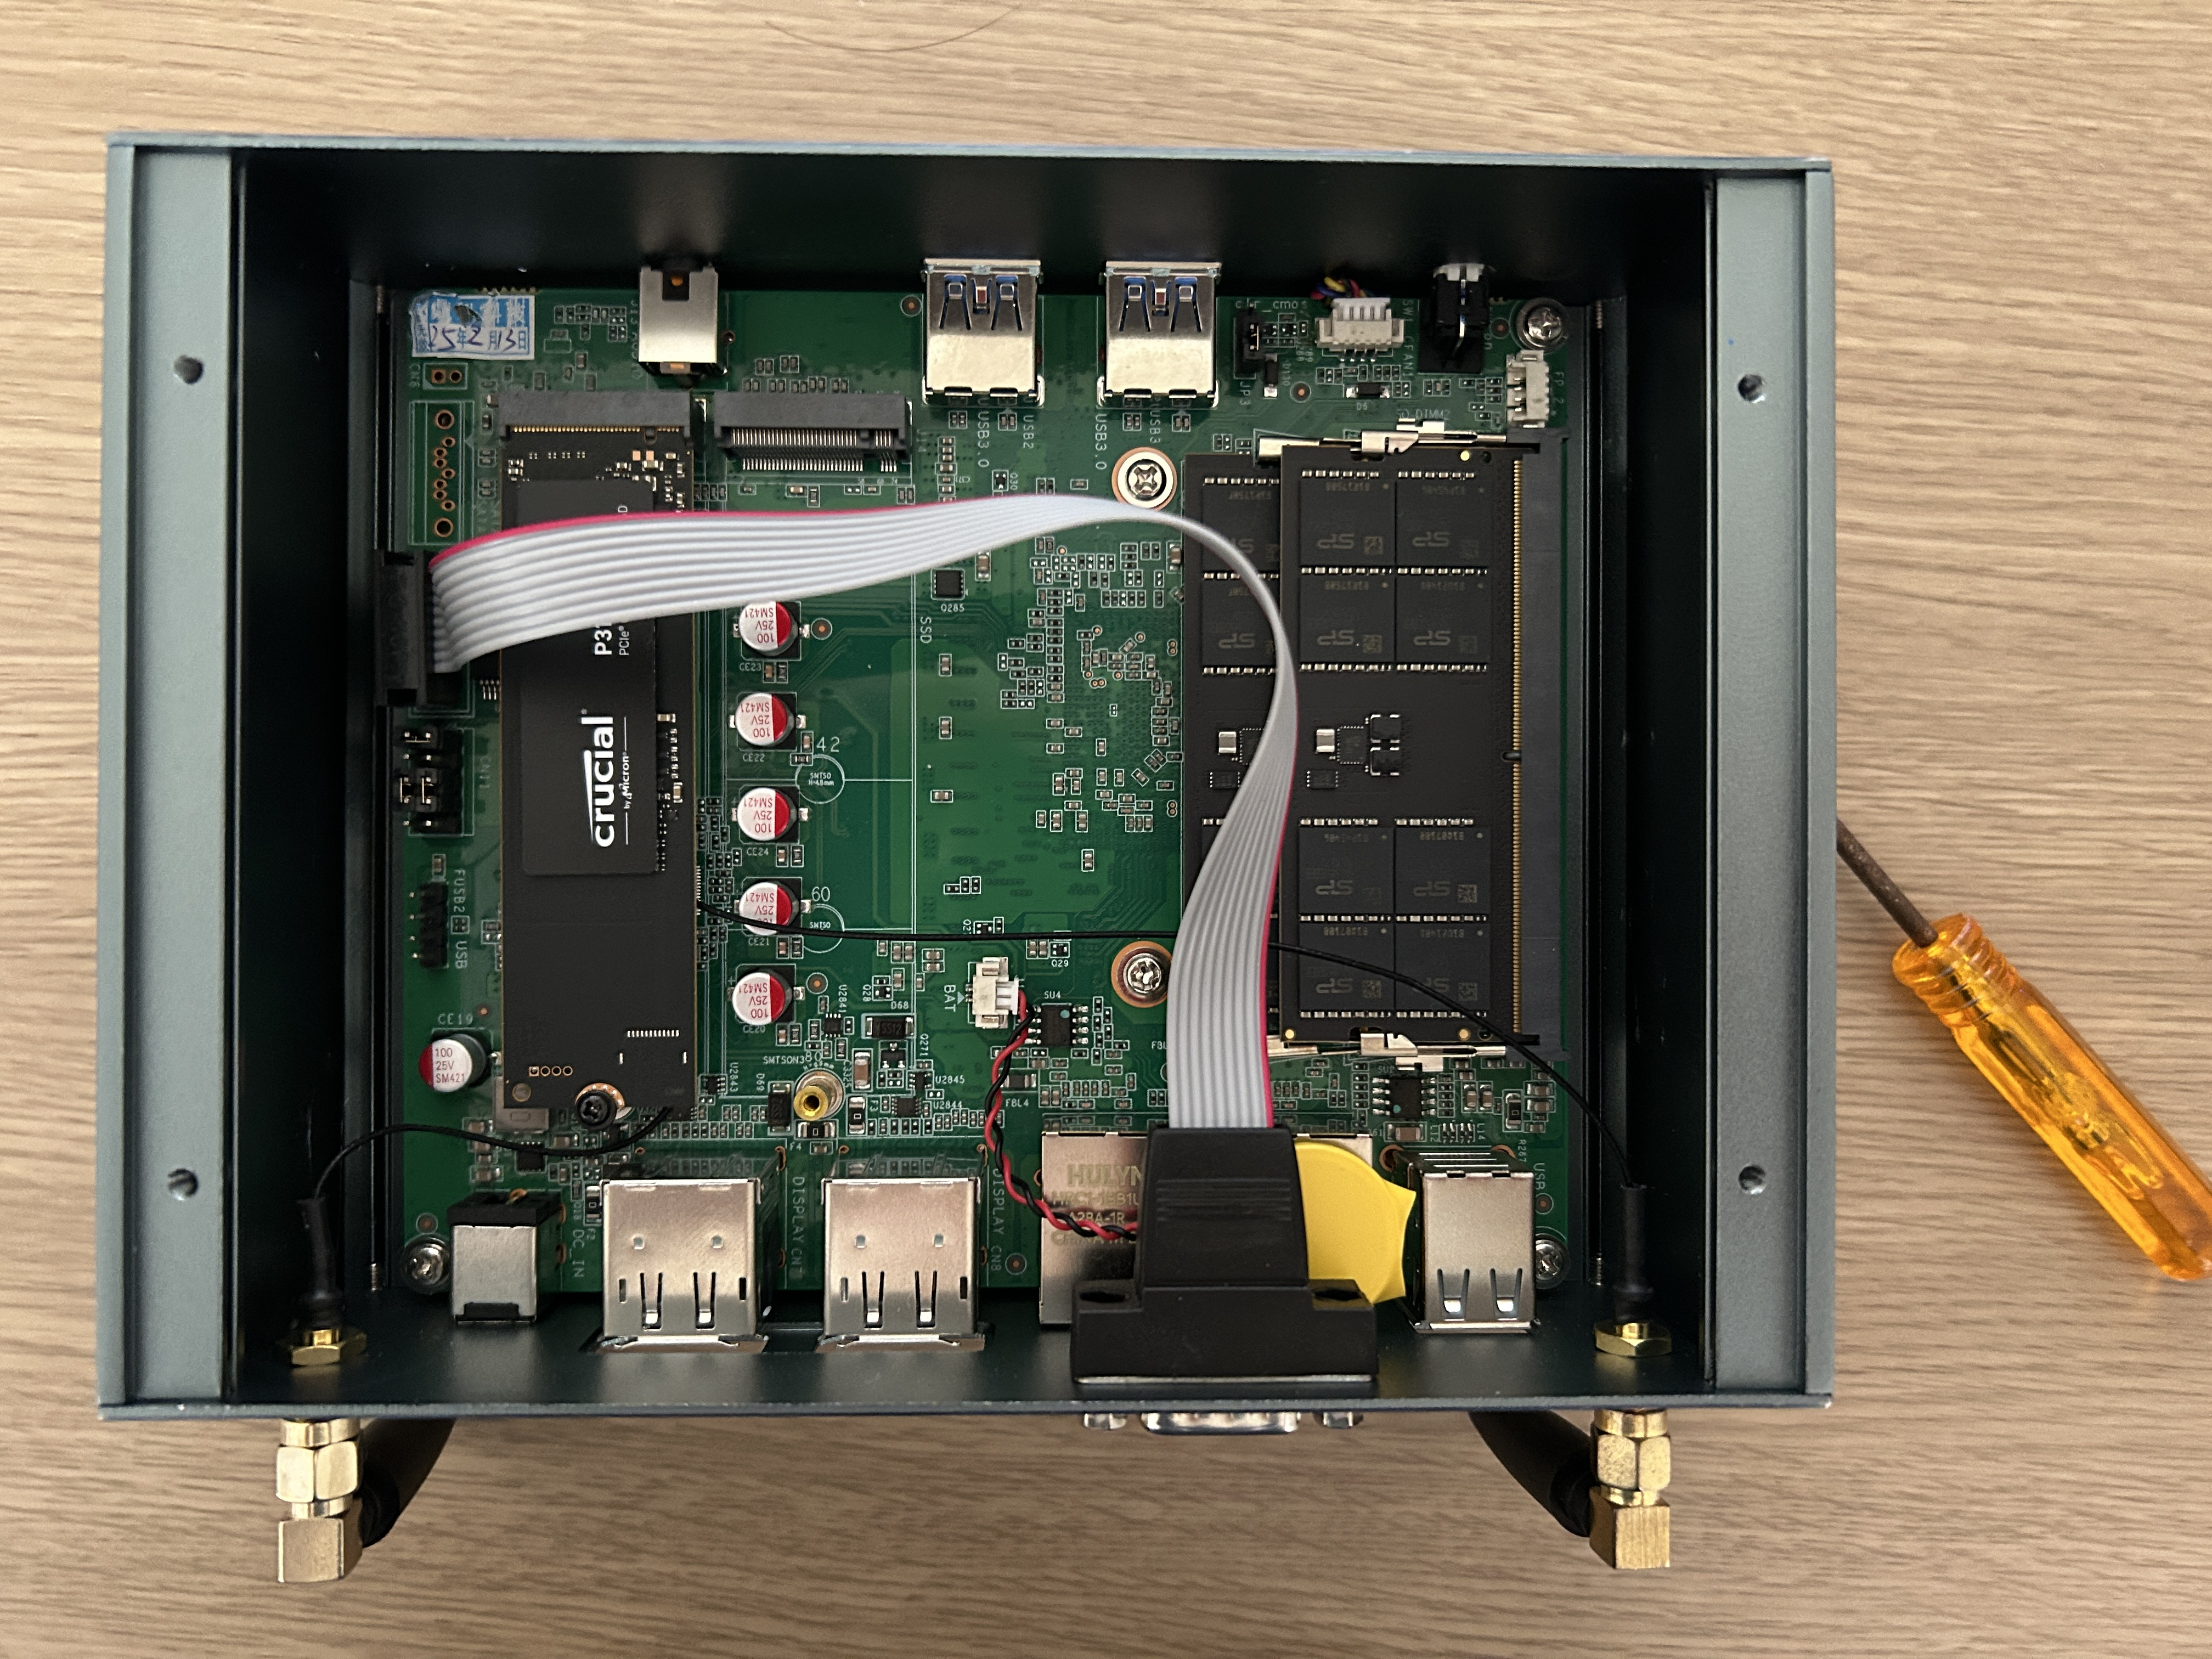
\includegraphics[clip=true,height=4.5cm,trim=0 0 500 0]{img/aiopcwa-internal-1.jpg}
   };
   \bndbox
  \end{scope}
 \end{tikzpicture}
 \newpage
 % install arch linux 1
 \begin{tikzpicture}
  \coorddecl

  \draw [
    xshift=51.5mm,
    yshift=20mm,
    line width=0.25mm,
    color=CampbellBrightGreen]
   (0mm,0mm) [rounded corners=0.5mm] rectangle (5.2mm, 18mm);

  \begin{scope}[on background layer]
   \node [anchor=center] at ($0.3*(ltpos) + 0.4*(rbpos)$) {
     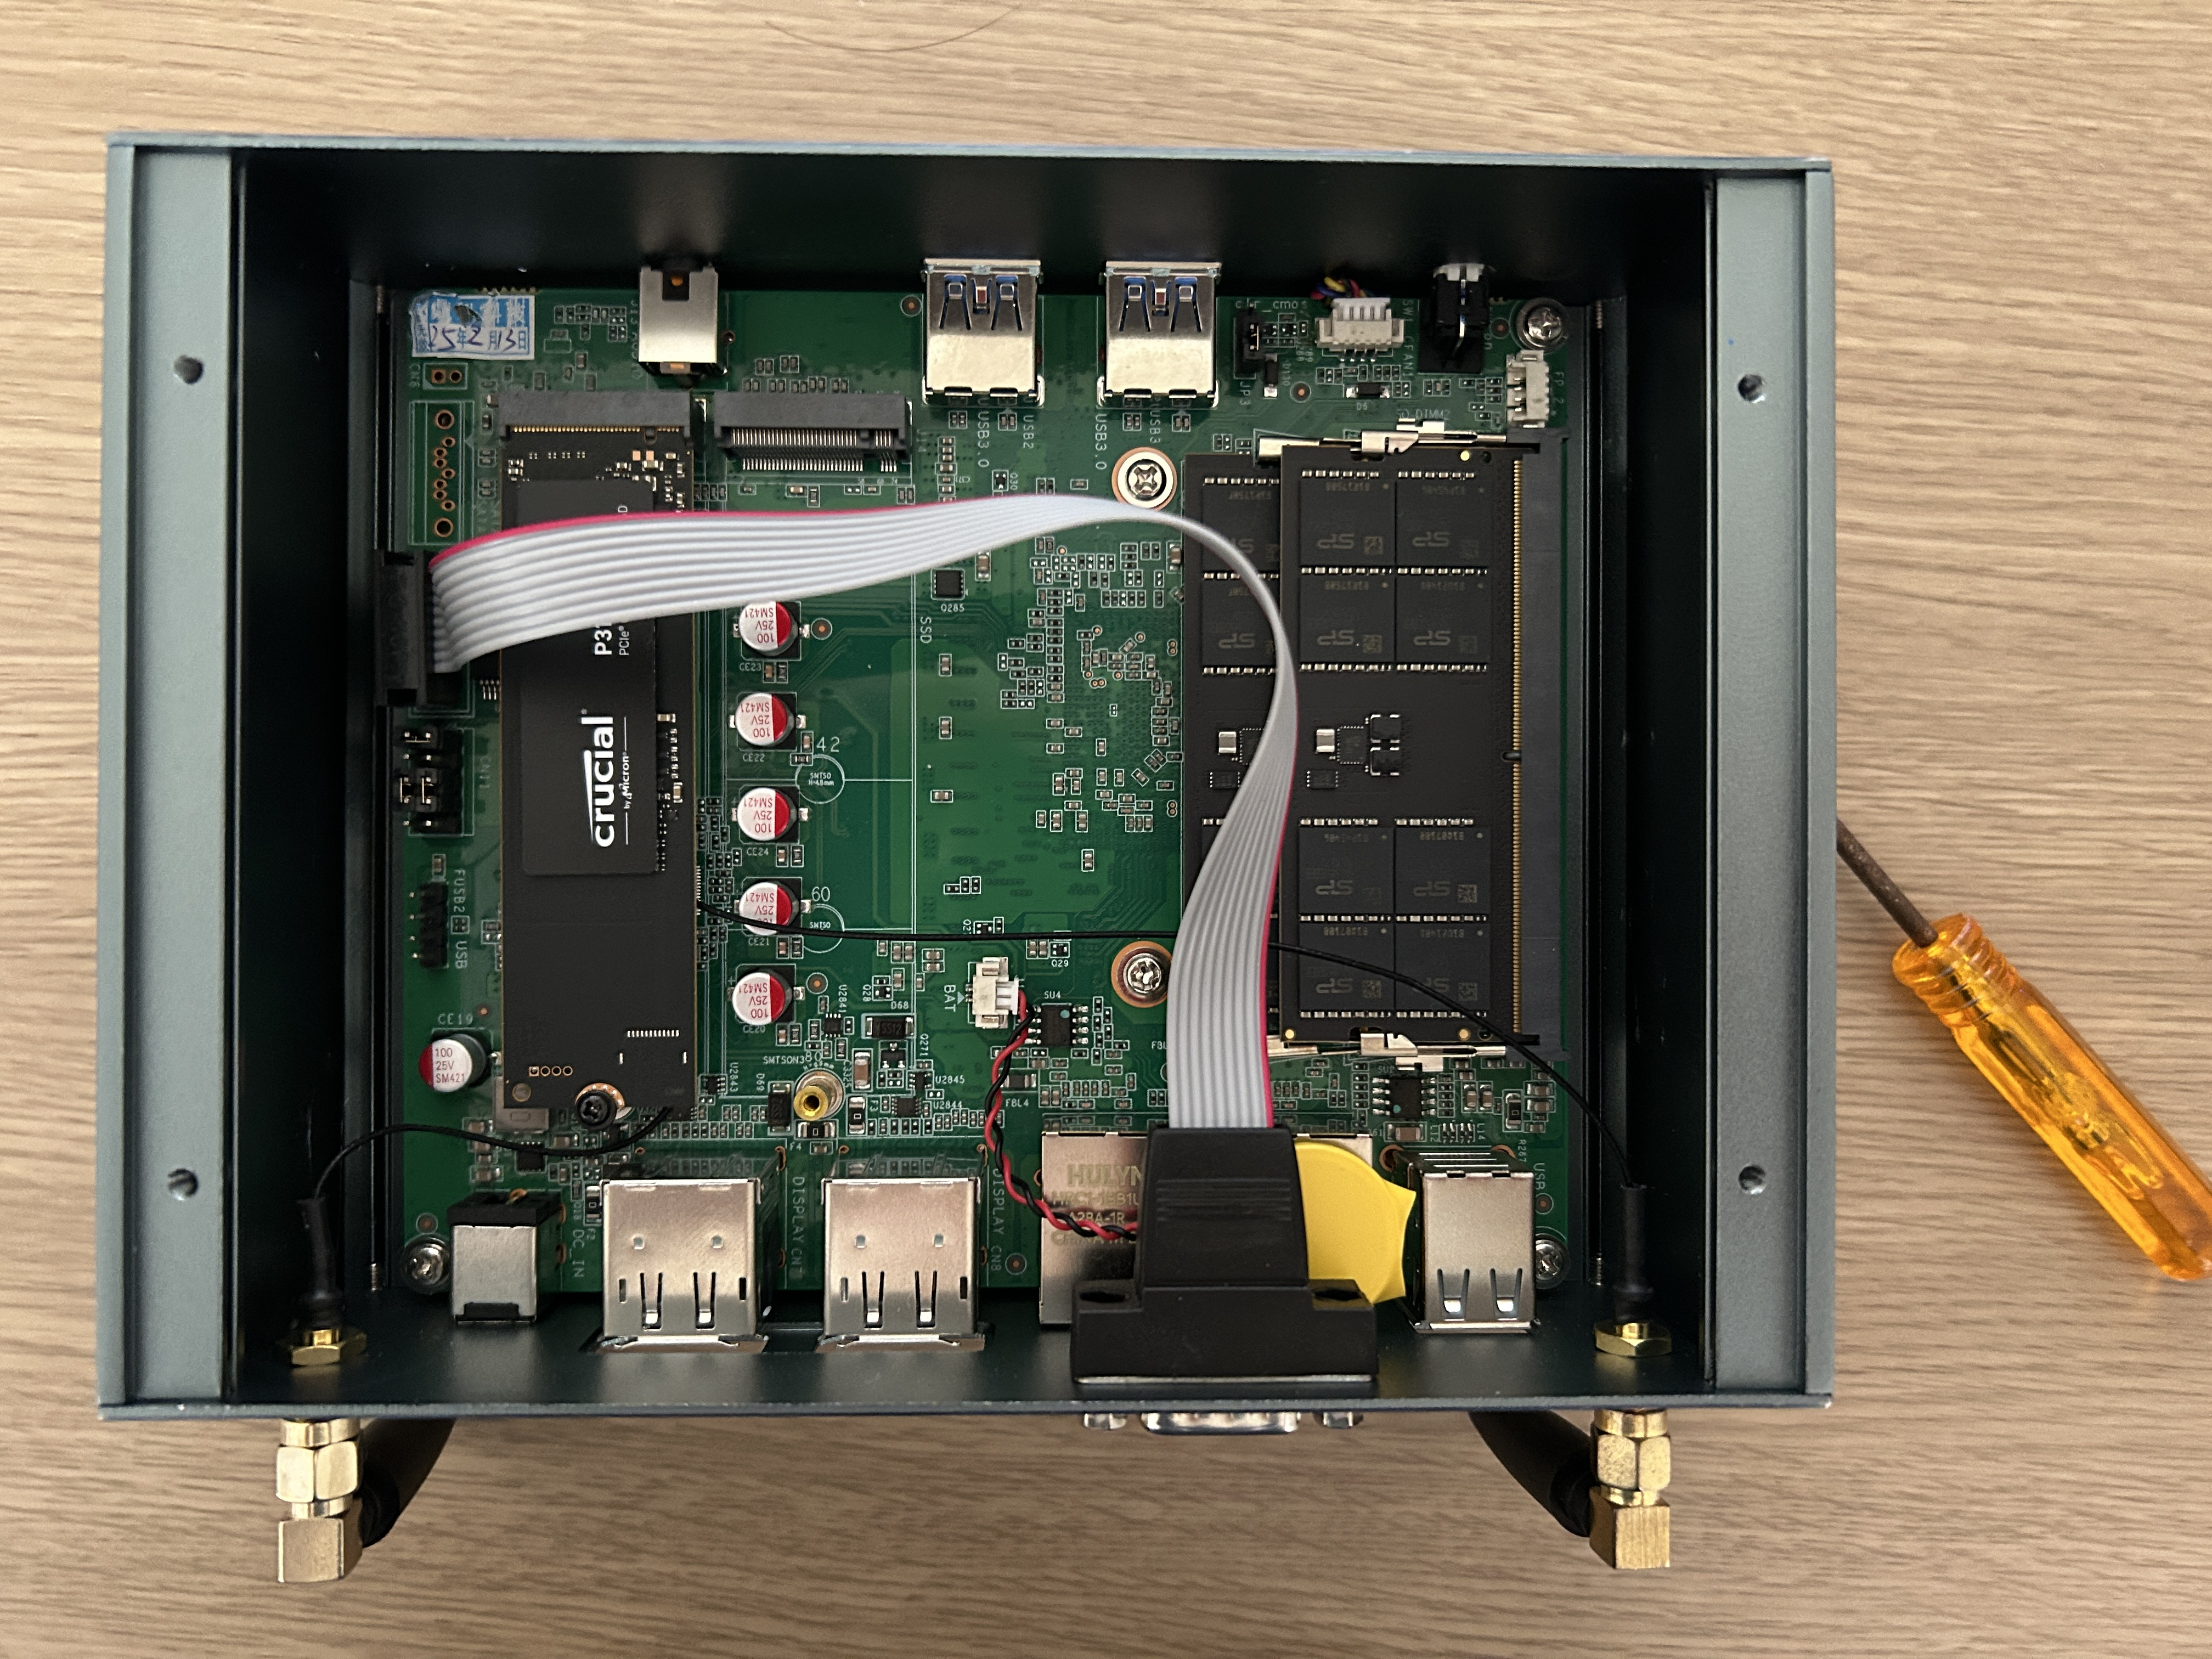
\includegraphics[clip=true,height=4.5cm,trim=0 0 500 0]{img/aiopcwa-internal-1.jpg}
   };
   \bndbox
  \end{scope}
 \end{tikzpicture}
 \newpage
 % install arch linux 3
 \begin{tikzpicture}
  \coorddecl
  \newcommand{\insarrow}{
   [xshift=38mm,yshift=40mm,rotate=90] (0mm,0mm) -- (5mm, 5mm)
    |- (18mm, 2.5mm) -- (18mm, -2.5mm)
    -| (5mm, -5mm) -- cycle}


  \draw [
    xshift=51.5mm,
    yshift=20mm,
    line width=0.25mm,
    color=CampbellBrightGreen]
   (0mm,0mm) [rounded corners=0.5mm] rectangle (5.2mm, 18mm);

  \begin{scope}
   \fill [color=CampbellBrightGreen] \insarrow;
  \end{scope}

  \begin{scope}[on background layer]
   \node [anchor=center] at ($0.3*(ltpos) + 0.4*(rbpos)$) {
     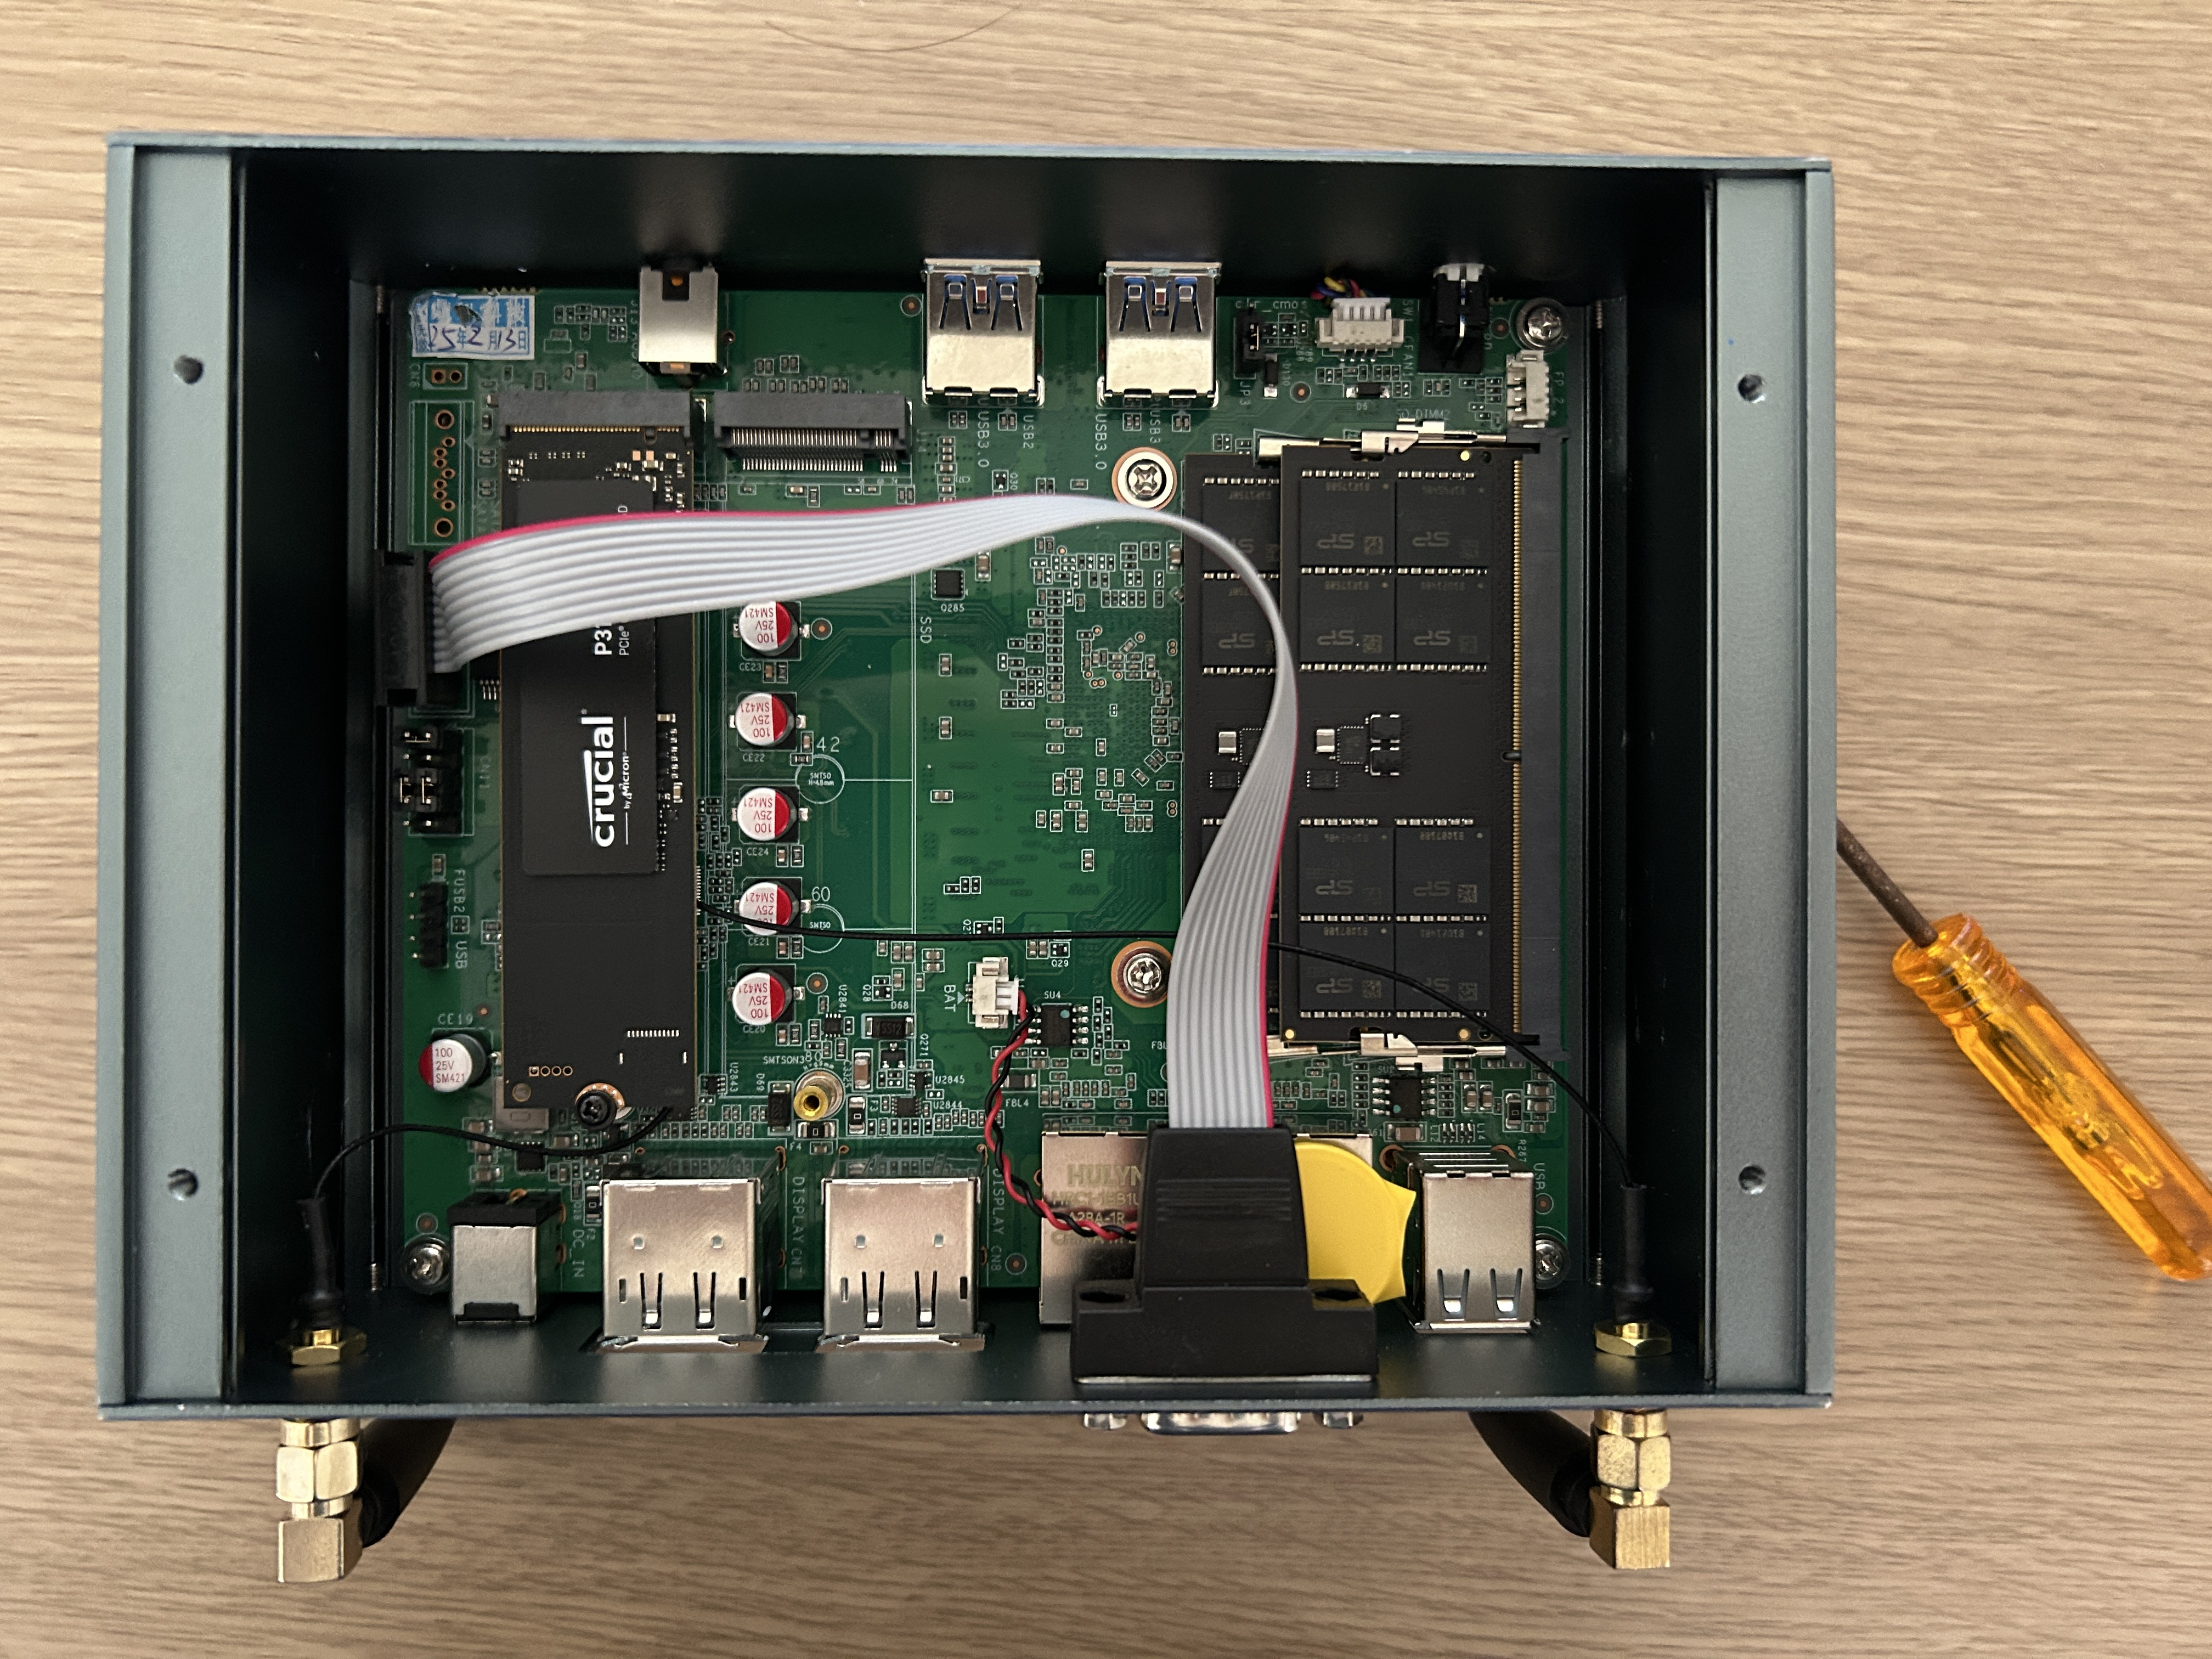
\includegraphics[clip=true,height=4.5cm,trim=0 0 500 0]{img/aiopcwa-internal-1.jpg}
   };
   \bndbox
  \end{scope}
 \end{tikzpicture}
 \newpage
 % insert usb 1
 \begin{tikzpicture}
  \begin{scope}[on background layer]
   \node [anchor=center] at ($0.5*(ltpos) + 0.5*(rbpos)$) {
     \includegraphics[height=6cm, page=10]{img/hw-img.pdf}
   };
   \bndbox
  \end{scope}
 \end{tikzpicture} 
 \newpage
 % insert usb 2
 \begin{tikzpicture}
  \begin{scope}[on background layer]
   \node [anchor=center] at ($0.5*(ltpos) + 0.5*(rbpos)$) {
     \includegraphics[height=6cm, page=11]{img/hw-img.pdf}
   };
   \bndbox
  \end{scope}
 \end{tikzpicture} 
 \newpage
 % insert usb 3
 \begin{tikzpicture}
  \begin{scope}[on background layer]
   \node [anchor=center] at ($0.5*(ltpos) + 0.5*(rbpos)$) {
     \includegraphics[height=6cm, page=12]{img/hw-img.pdf}
   };
   \bndbox
  \end{scope}
 \end{tikzpicture}
\end{document}

% vi: se ts=1 sw=2 et:
